\section{Main elements of the user interface}
\label{sec:user_interface}
This section gives an overview of the main user interface elements and features of \pkg{RKWard}\footnote{
    The \proglang{R} script and data for automatic demonstration can be found in the accompanying zipped file ``examples.zip''.
}.
For a use case oriented example of an \pkg{RKWard} session, see Section~\ref{sec:using_RKWard}.

The default layout\footnote{
 Many aspects of the \pkg{RKWard} GUI can be customized by the user. For simplicity we will
 describe the default appearance of \pkg{RKWard}, only. 
} of the main application window is divided into five
parts, as depicted in Figure~\ref{fig:main_window}. The top of the window is occupied by menu bar and toolbar 
(Figure~\ref{fig:main_window}A). The content of both bars is partially context
sensitive, e.\,g., the ``Edit'' menu will offer
one set of actions when the current document window is a data editor,
and another set of actions for a \proglang{R} script
editor window. To ease orientation, all top level menus remain
persistent, even if no actions are available for that menu in the
current context. The menu bar of the main window is also the central
access point to most data import, manipulation, analysis, and
visualization features (see Section~\ref{sec:analyzing_data}) for which \pkg{RKWard} provides a GUI
interface.

\begin{figure}[h!]
 \centering
 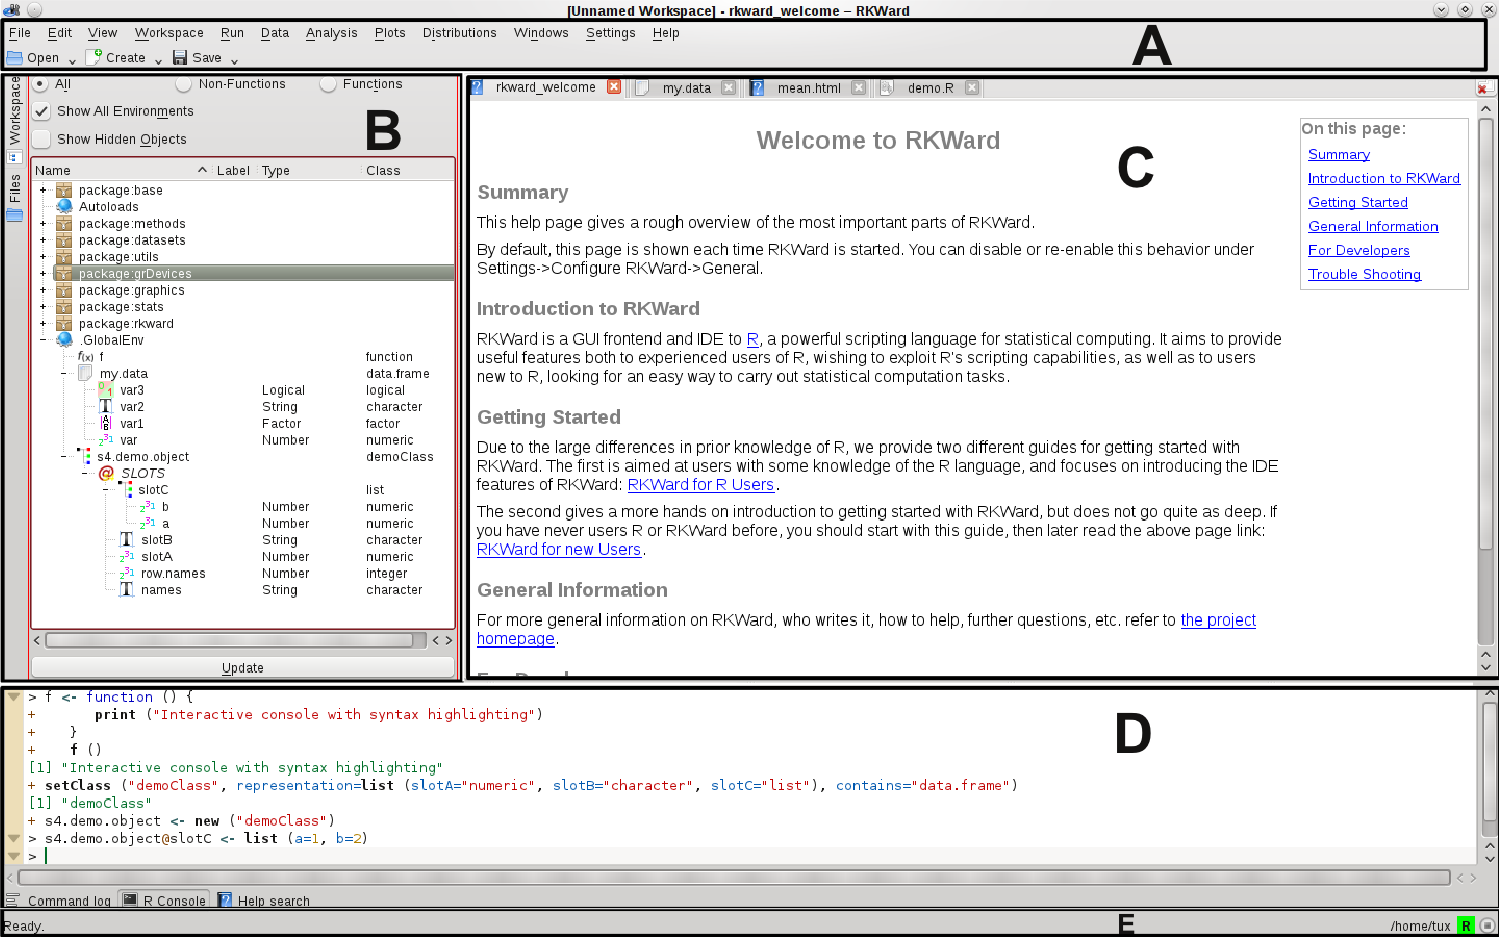
\includegraphics[width=15.450cm]{./figures/main_window.png}
 \caption{Default \pkg{RKWard} main window after start up. 
A) Menu bar and toolbar, B) tool panel showing workspace browser, C) document view area, showing
different documents (welcome message, \code{data.frame} ``my.data'', ``mean'' help page, \proglang{R}
script ``demo.R''), D) tool panel showing embedded \proglang{R} console, and E) status bar with an option to
stop running processes. Panels B and D can be resized or collapsed. The red border around B indicates that the
workspace browser is the active interface element.}
 \label{fig:main_window}
\end{figure}

A status bar is shown at the bottom of the window (Figure~\ref{fig:main_window}E). It displays (from
right to left) a ``Stop''-button to interrupt the current computations,
the status of the \proglang{R} engine (busy or idle), the
current working directory, and a multi purpose region for additional
information on some menu items and other GUI elements, visible when
hovering the mouse pointer over them.

The \pkg{RKWard} GUI generally follows an MDI (multiple document interface) approach.
Document windows (object summaries, Section~\ref{sec:workspace_browser_object_viewer};
    script editors, Section~\ref{sec:code_editor}; spreadsheet-like data editors, Section~\ref{sec:spreadsheet};
    results output, Section~\ref{sec:results_output}; help pages, Section~\ref{sec:help_system}; and also
    \proglang{R} on-screen graphics devices, Section~\ref{sec:plot_previews}) 
are arranged in a TDI \citep[tabbed document interface; see e.g.][]{Hopkins2005, MDN2010, KimLutteroth2010}
in the central area (Figure~\ref{fig:main_window}C). The order
of tabs can be conveniently re-arranged using drag \& drop.

Additionally, several tool windows are available form resizable sub-panes at the four sides\footnote{
    This combination of a tabbed-document interface and sub-panes is sometimes referred to as an ``IDE-style'' interface, due to its
    usage in popular IDEs such as \pkg{Eclipse} \citep{Eclipse} or \pkg{KDevelop} \citep{KDevelop}.
}. By default, the
left panel (Figure~\ref{fig:main_window}B) contains a file browser (see Section~\ref{sec:further_tool_windows}) and a
workspace browser (see Section~\ref{sec:workspace_browser_object_viewer}), the
bottom panel (Figure~\ref{fig:main_window}D) contains a command
log (Section~\ref{sec:further_tool_windows}), an \proglang{R} console
(Section~\ref{sec:using_R_console}), and a help search (Section~\ref{sec:help_system}) window. The top and right sub-panes are
not populated by default.

Users can also detach all types of document windows and tool windows from the main application window, which will
then appear as independent windows, managed by the window manager, or re-attach them to the main window.
This is to allow users to take advantage of an SDI (single-document interface), where useful, such as the ability to view any two
documents side-by-side, or to make better use of multiple displays. On{}-screen
graphics device windows are created detached by default, but can 
be attached to the document view area of the main window.

Windows can be selected (or shown / hidden) using a mouse device with point \&
click, as well as using a series of keyboard shortcuts (defined by
default) for activating specific tool windows, or for cycling through all windows
in the order of most recent usage\footnote{
    This uses the shortcut ``Ctrl+Tab'' by default, and behaves similar to the ``Alt+Tab''
    feature of common window managers. The difference is that this cycles through \pkg{RKWard} windows,
    only, including both detached windows, and windows which are attached inside the main application
    window.
}.

All key bindings can be configured from the GUI via ``Settings$\rightarrow$Configure Shortcuts''. 
However, for technical reasons only the shortcuts of currently active components 
will be listed. Thus, for example, to
configure data editor shortcuts, one has to open a data editor first and
then to select ``Settings$\rightarrow$Configure Shortcuts''. Since \pkg{RKWard} relies on the 
\pkg{RKWard} editor component,
shortcuts for the script editor (Section~\ref{sec:code_editor}) are managed separately via 
``Settings$\rightarrow$Configure Editor$\rightarrow$Shortcuts''. On most systems, it is also
possible to configure shortcuts by right-clicking on the respective
menu item.

The choice of available actions on the toolbar can be
configured via ``Settings$\rightarrow$Configure Toolbars''. Further, it is possible to add and remove sets
of data manipulation and analysis features from the GUI, using
``Settings$\rightarrow$Configure RKWard$\rightarrow$Plugins''.

\subsection{Workspace browser and object viewer}
\label{sec:workspace_browser_object_viewer}

The workspace browser (Figure~\ref{fig:main_window}B) allows to view
and manipulate \proglang{R} objects, similar
to a regular file-system browser. This includes both, user objects
(data, functions, environments) in \code{.GlobalEnv} and non-user objects in other environments in the
\proglang{R} search path (typically,
\proglang{R} package environments). Objects are shown
in a hierarchical tree structure. For instance, an object of class
\code{list} can be expanded to show all contained objects 
by clicking on the $+$ symbol left of the object name.
The basic type of each object is indicated by specific icons\footnote{The workspace browser 
indicates the types ``Number'', ``Factor'', ``String'', and ``Logical'' for the \code{data.frame} 
``my.data'' (Figure~\ref{fig:main_window}B).}. 
Further information on each object can be seen by hovering the mouse
pointer over the respective icon. A tooltip window will appear,
including information such as dimensionality or function arguments,
depending on the type of object. Further, objects inside \code{.GlobalEnv} can be
removed, renamed, and edited from the context menu.

Several actions are available from a context menu (after right-clicking
on the object names), depending on the type of object. These allow to search the
\proglang{R} help for information on that object, to
open a window with detailed information on the object, to delete, rename or copy the object to a new symbol name, or to
copy it to \code{.GlobalEnv}. Further, the context menu allows to open
supported types of objects for editing (see Section~\ref{sec:spreadsheet}; currently, only
\code{data.frame}s can be edited, and only while they exist in \code{.GlobalEnv}). 
Selecting ``View'' from the 
context menu opens a new window in the
document area, containing basic information on the object as well as 
tabs which show the output of
\code{print()} and \code{summary()} calls.

Literally hundreds or even thousands of objects are present in a typical
\proglang{R} session. This can be overwhelming at
first, therefore, the workspace browser has options to show only a certain
subset of objects, e.\,g., only functions or only data objects, including
or excluding hidden objects (object names starting with a 
``.''), or showing only the contents of \code{.GlobalEnv} as
opposed to all environments in the search path.

An object list similar to the workspace browser (but showing only 
\code{.GlobalEnv} by default) is also used in several places for the
selection of objects to work with, e.\,g., in an analysis plugin (see Section~\ref{sec:analyzing_data}).


\subsection{Code editor}
\label{sec:code_editor}

\pkg{RKWard} comes with an advanced
\proglang{R} script editor, based on the
\pkg{KDE} advanced text editor component (\pkg{Kate}; \url{http://kate-editor.org/}). Features of this
editor include syntax highlighting (both on screen and in printouts; for
\proglang{R} and many other script types), code
folding, block-wise indentation adjustments or commenting, automatic
brackets, search and replace with plain text or regular expressions,
and many more. Further, \pkg{Kate} can be extended by 
customized actions implemented in \proglang{ECMAScript} \citep{KateScriptedActions}.
The editor automatically saves snapshots of the
currently edited files at configurable intervals. 

For interaction with \proglang{R}, the editor has
predefined shortcuts (and toolbar icons) for submitting the current line, the current 
selection, predefined blocks, or the entire document to the
\proglang{R} engine for evaluation. It also 
offers object name completion and function argument hinting 
(Figure~\ref{fig:code_hinting}A and B) based on the objects present in
the \proglang{R} workspace\footnote{The object name
completion and function argument hinting features in \pkg{RKWard} predate the
inclusion of similar features into the core
\proglang{R} distribution. For this reason, they are
technically based on different mechanisms.}. A further feature specific
to the \proglang{R} language is the
``Paste Special'' action, which allows to
paste the clipboard content (e.\,g., from a separate spreadsheet
application) as a single string, vector, or matrix, suitable
for inclusion in an \proglang{R} script, optionally
transforming it in advance (Figure~\ref{fig:special_paste}).

\begin{figure}[t!]
 \centering
 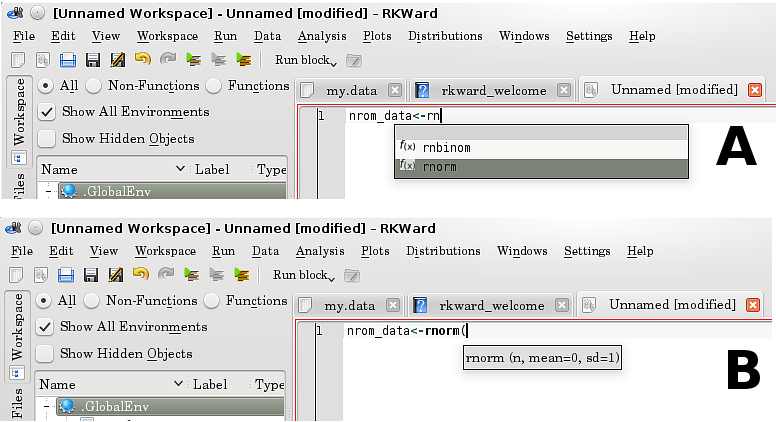
\includegraphics[width=15.5cm]{./figures/code_hinting.png}
 \caption{Code hinting features of the script editor. The script editor is able to hint A) \proglang{R} object names
and B) function arguments.}
 \label{fig:code_hinting}
\end{figure}

\begin{figure}[t!]
 \centering
 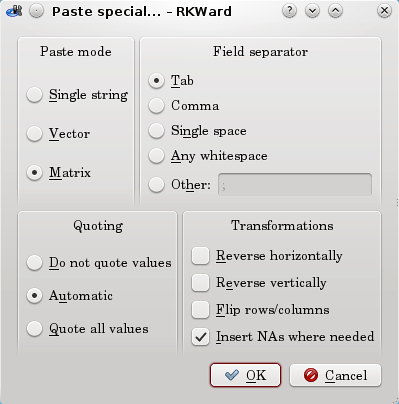
\includegraphics[width=9.0cm]{./figures/special_paste.png}
 \caption{Paste special dialog. This tool allows to paste data (e.\,g., tabular, text) from the clipboard, directly to an 
 \proglang{R} script and therefore accelerates the work process with data from different sources 
 like spreadsheet applications.
}
 \label{fig:special_paste}
\end{figure}

Script editor windows can be created by opening an existing
\proglang{R} script file from the file browser, the
``File'' menu, or by creating a new empty script. It can
also be invoked from \proglang{R}, e.\,g., using the
\code{file.edit()}, \code{file.show()}, or \code{fix()}
commands.

\subsection[Using the R console]{Using the \proglang{R} console}
\label{sec:using_R_console}
For users with knowledge of \proglang{R}, \pkg{RKWard} provides direct access to the
embedded \proglang{R} engine in the
\proglang{R} console tool window. It is important to understand that technically this is an
emulation of \proglang{R} running in a console
session, not a real \proglang{R} session. This leads to a few subtle
differences, e.\,g., with respect to the command history feature in
\proglang{R}.

However, for most purposes \pkg{RKWard}'s \proglang{R} console can be used exactly
like \proglang{R} running in a terminal. Adding to that, it provides many of the
features which are also available in the code editor (see Section~\ref{sec:code_editor}).
Most prominently, it supports syntax highlighting, code
folding, function argument hinting, object name completion, and pasting
vector or matrix data directly from the clipboard.

By default, any code that is submitted to the
\proglang{R} engine from the code editor or from help
pages, is sent through the \proglang{R} console.
However, it can be configured to be submitted in the background,
instead.


\subsection{Spreadsheet-like data editor}
\label{sec:spreadsheet}

Historically, one of the earliest
features of \pkg{RKWard} is a built-in spreadsheet-like data editor.
Currently, editing \proglang{R} objects of type
\code{data.frame} is possible. In contrast to the \code{data.frame} editing shipped
with the \proglang{R} core distribution, this editor
gives the illusion of ``in-place'' editing of data. New \code{data.frame}s can
be created and opened from the GUI, and existing objects can be opened
for editing from the workspace browser. For opening objects from
\proglang{R} code, the function \code{rk.edit()} can be used.
Figure~\ref{fig:data_editors} shows multiple \code{data.frame}s open for editing.

\begin{figure}[b!]
 \centering
 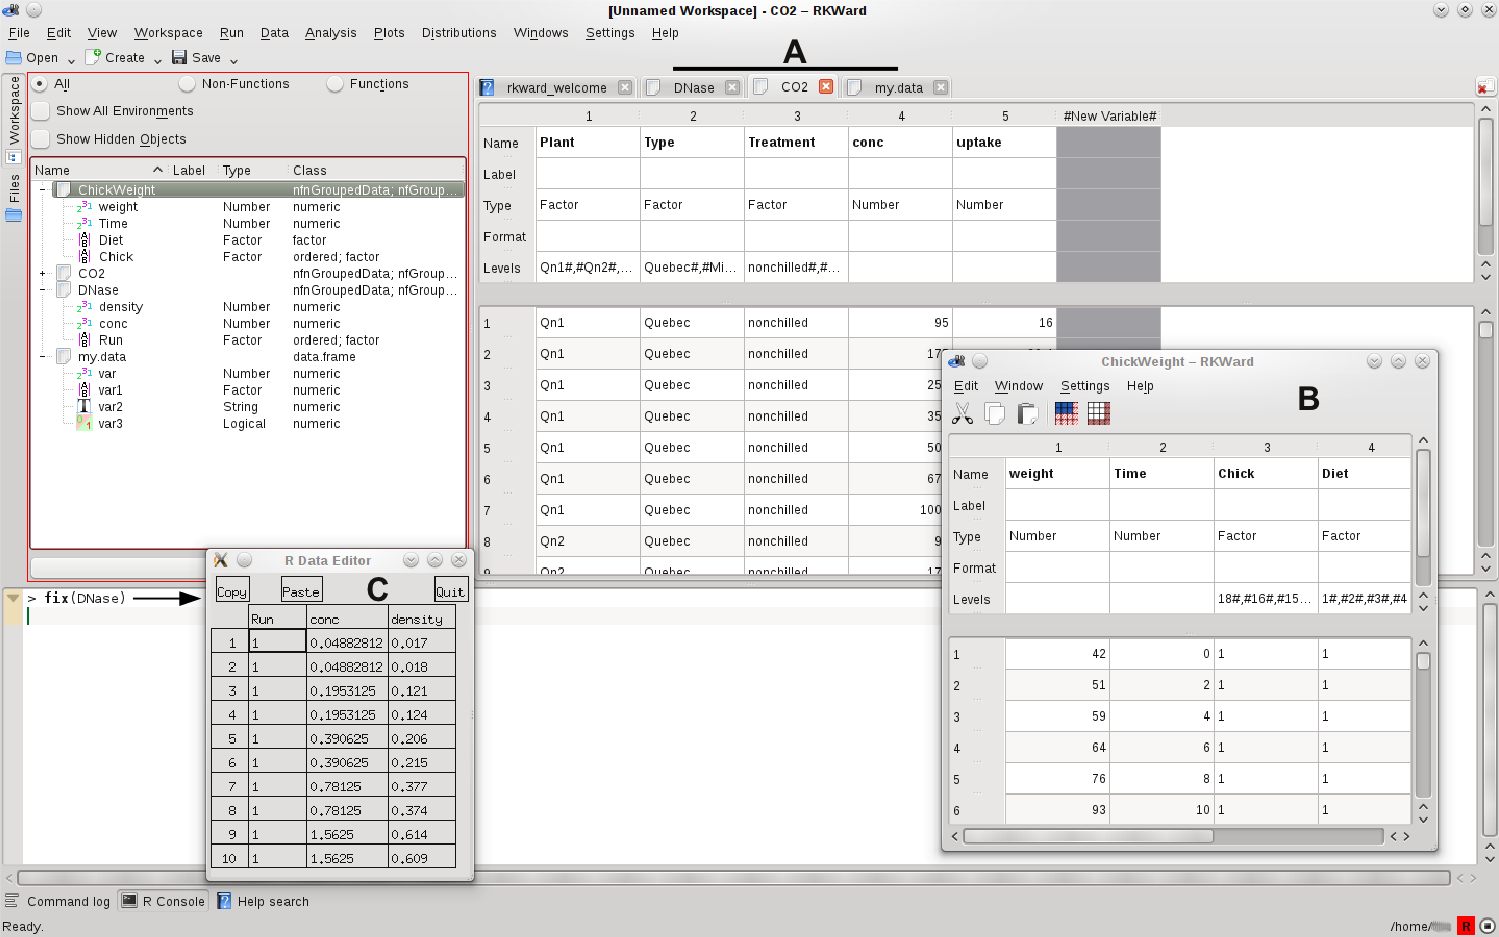
\includegraphics[width=15.5cm]{./figures/data_editors.png}
 \caption{\pkg{RKWard} with several \code{data.frame}s in use at the same time. A) 
  One \code{data.frame} (\code{CO2} data of the \pkg{datasets} package) is opened for editing in the main window. Two further \code{data.frame}s
  are opened in the background in tabs. 
  B) Another \code{data.frame} (\code{ChickWeight} data of the \pkg{datasets} package) is opened as detached window. 
  C) \proglang{R}'s standard data editing features (e.\,g., \code{fix()}, \code{edit()}) 
  are also usable within an \pkg{RKWard} session. In this example \code{fix(DNase)} 
  was invoked from the console (arrow).}
 \label{fig:data_editors}
\end{figure}

Metadata on each column of a \code{data.frame} (i.\,e., name of the column, data
type, and potentially data labels) is shown in the upper portion of
the data editor, and can be manipulated there, while the data itself is
shown in the lower portion. The upper portion can be hidden using a
slider, to save space for the display and editing of actual data.
Similarly, an editable column showing the row names of the \code{data.frame}
can be shown or hidden separately from the data.

For columns of type \code{factor}, factor levels can be edited by double-clicking on the
``Levels'' row of the meta information. Levels can also be assigned to other types of
variables, but only for consecutive integer values. These levels will
be displayed instead of the underlying value, if applicable. Each
column can also be assigned an arbitrary descriptive
``Label'', which is stored in
\proglang{R} as an attribute of the column.

Contrary to many other editors, the data editor in \pkg{RKWard} does not
automatically convert data types of columns. For instance, if a
non-numeric string is entered into a cell of a numeric column, the data
type of the column remains numeric, and the entered value is
highlighted in red. Internally, the invalid cell is set to \code{NA}.
The entered value is stored separately, in an attribute of the column.
The rationale for this approach is that it offers protection against
accidental, and probably undetected, conversion of data types. The
user can manually convert the storage mode of a column by simply
selecting a different data type in the ``Type'' row of the meta information.

The data editor supports insertion and deletion of rows or columns at 
arbitrary positions. Rows (columns) can also be added at the bottom 
(right) by simply entering data into the trailing row (column) shown in
gray. Copy \& paste is supported, where the area affected by paste
operations can optionally be constrained to the selected region, or to
the dimensions of the table. The data editor can also be set to read-only
mode to examine data objects.

In the context of data editing, it is noteworthy that
\pkg{RKWard} supports working with multiple objects simultaneously, rather than
limiting actions to a single active \code{data.frame}, as with e.\,g., \pkg{Rcmdr} or
\pkg{DeduceR}. Given this non-modal interface design, multiple data editor
windows can be opened at once (Figure~\ref{fig:data_editors}).

\subsection{Handling, manipulating, and analyzing data}
\label{sec:analyzing_data}

Dealing with data -- i.\,e., importing, transforming, filtering, analyzing, and visualizing  --
is the core strength of \proglang{R}, and one central goal of
\pkg{RKWard} is to make the most of this functionality available to a broader
audience by providing it in the form of easy to use GUI dialogs. Since
the data handling functionality itself is provided by
\proglang{R} and its numerous add-on packages, this
can basically be accomplished by defining GUI dialogs, generating
\proglang{R} code according to the settings made in
the GUI, and having the generated code evaluated by the
\proglang{R} engine. 
This general pattern, implemented as plugins, is the
basic recipe for most of the functionality provided by \pkg{RKWard}
(see the technical supplement to this article for details on the definition of plugins). For
the purpose of this article we will look at the standard
elements of data handling functions by an example of importing comma-separated values (CSV)
data\footnote {
  Note that on purpose, \pkg{RKWard} does not have its
  own file format for data import and export, but rather uses
  \proglang{R} workspaces as default data format. Additionally, it is possible
  to import data from several sources as described in this section. Of course, further formats can
  also be imported using copy \& paste (see Sections~\ref{sec:code_editor} and \ref{sec:spreadsheet}), or by
  manually entering appropriate \proglang{R} commands in
  the \proglang{R} console (Section~\ref{sec:using_R_console}).
}. Further examples are given in Section~\ref{sec:using_RKWard}.

At the time of this writing, \pkg{RKWard} provides support for importing \proglang{SPSS},
\proglang{Stata}, and ``delimited text'' data. Internally, \pkg{RKWard}
relies on standard \proglang{R} functions and the package \pkg{foreign}
\citep{Murdoch2002} for reading these data files. To import CSV data,
select ``File$\rightarrow$Import format$\rightarrow$Import Text$\rightarrow$CSV''
data from the menu. This will open the dialog shown in
Figure~\ref{fig:CSV_import}. The central area of this dialog provides 
options to control the import. The 
``File name'' field is highlighted, to indicate that
it is required to specify a file before the dialog can proceed.
Further options are available from the tabbed pages of the central area.

\begin{figure}[b!]
 \centering
 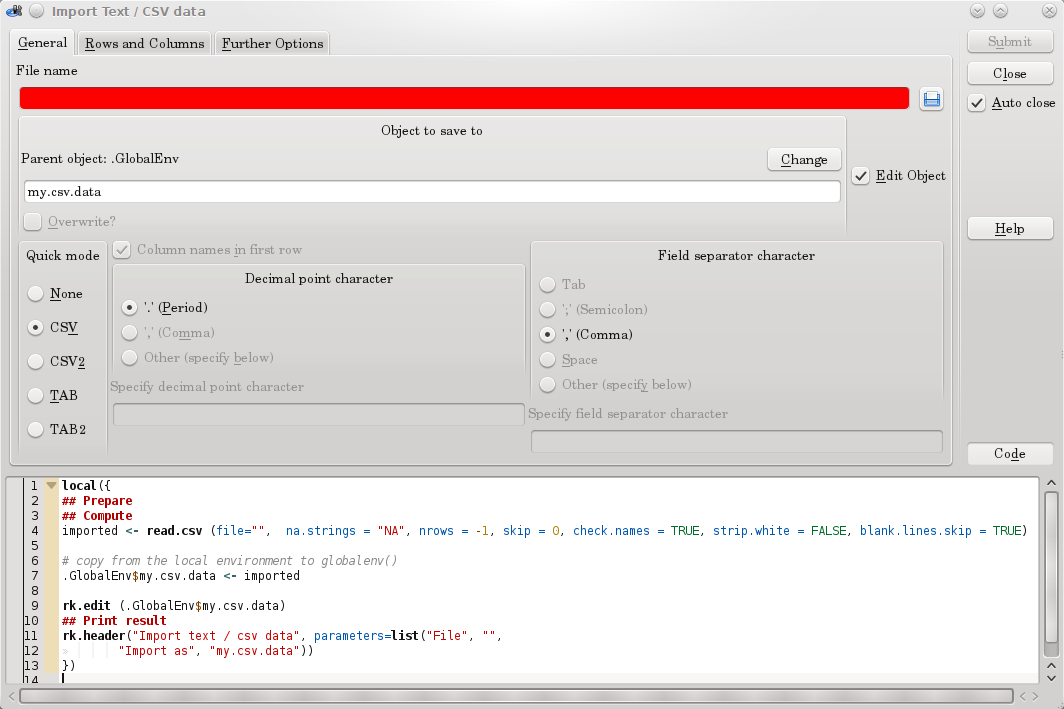
\includegraphics[width=14.99cm]{./figures/CSV_import.png}
 \caption{General data import dialog. Useful defaults for a variety of formats can
  be set using the ``Quick Mode'' selector on the left. Further customizations can be done
  from the ``Rows and Columns'' and ''Further Options'' tabs. The 
  code in the bottom area can be copied and used for other purposes.}
 \label{fig:CSV_import}
\end{figure}

The right-side area is common to all data handling
dialogs. Here the ``Submit'' button is used
to start the import action. It is enabled once all required
settings have been made, i.\,e., in this case, once a file name has been
selected. The ``Close'' button will close the
dialog without taking any action.

The bottom area optionally shows the \proglang{R}
code corresponding to the current settings  which will be run
upon pressing the ``Submit'' button (see Section~\ref{sec:importing_data} for generated \proglang{R} code). 
The code display is hidden by default and can be revealed using
the ``Code'' button. This 
generated code display is updated dynamically as the user changes settings, allowing
to see the effect of each change instantly.

Most data handling functions will produce some output, which is
sent to the output window. From there it is possible to repeat the
action by clicking on the ``Run again''-link
(see Section~\ref{sec:results_output}).

\subsection{Graphics window and plot previews}
\label{sec:plot_previews}

For plotting, \pkg{RKWard} relies on the graphics capabilities provided by
\proglang{R}. All \proglang{R}
devices, including on{}-screen devices, can be used in the regular way.
However, for the \code{X11()} and \code{windows()} devices, \pkg{RKWard} adds a menu
bar and a toolbar to the device windows (on the Microsoft Windows platform,
replacing the default menu bar provided by the device). The menu
bar and toolbar give access to a number of different functions,
including GUI dialogs for exporting the current plot,
and adding a grid to an existing plot 
(works on only certain types of plots).

Further, a history mechanism is provided,
which stores created plots automatically and allows to navigate
back to earlier plots (Figure~\ref{fig:plot_history}). 
The history is available as a drop-down list of the plot calls as well as using typical ``back''
and ``forward'' buttons on the toolbar.
The maximum number
of plots to record, as well as the maximum size of each individual plot,
is configurable from the settings menu. This plot history is shared
between all open on{}-screen device windows, yet they behave
independently. For example, if multiple devices display the same
plot, any modification (including deletion) of the plot on one device
renders its instances on other devices as ``new'' and hence can be added
back to the plot history. In addition, duplicating or closing a device
window records any unsaved plots to the history.

\begin{figure}[b!]
 \centering
 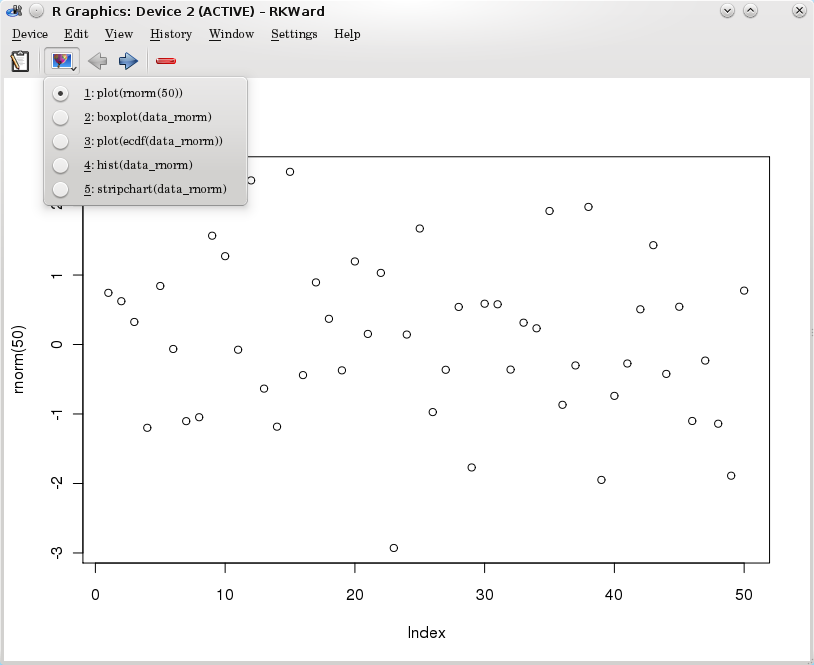
\includegraphics{./figures/plot_history_cropped.png}
 \caption{On{}-screen graphics device window in \pkg{RKWard}. The plot history is 
  available as a drop-down list, allowing to jump directly to a previous 
  plot. In this example, five different plots were performed on the same data 
  set of a random sample (\code{rnorm()}). The plot can be 
  exported via ``Device$\rightarrow$Export'' as described in Section~\ref{sec:create_plot}.
}
 \label{fig:plot_history}
\end{figure}

Further, \pkg{RKWard} provides access to different plotting functions using GUI dialogs,
available from the ``Plots'' menu. Wherever appropriate, \pkg{RKWard} supports a ``plot
preview'' feature. When the ``Preview'' box of
the respective dialog is checked, a device window is opened, which
shows the plot as it would be created with the current settings (see Section~\ref{sec:create_plot} for an example). The
preview is updated automatically as the user makes changes, allowing to
see the effect of each setting instantly\footnote{The preview is
updated asynchronously to keep the GUI responsive; see also the technical supplement to this article.}. For example, the
central limit theorem plugins
under the ``Distributions'' menu can be very helpful to dynamically ``show''
the convergence in distribution while teaching. For the sake of simplicity, such preview plots are not added to
the history.

\subsection{Results output}
\label{sec:results_output}

While all basic mechanisms of
capturing and documenting \proglang{R} output can also
be used, \pkg{RKWard} provides a dedicated output file and a output
window for documenting the results. All GUI-driven data handling
functions (see Section~\ref{sec:analyzing_data}) write their output to this file. 
The same applies to error messages, in case a plugin fails to perform its task.
The output is presented in a journal format\footnote{Note: The font size of the output can be adjusted
from the menu. 
}. All results are presented
sequentially with the last performed task at the bottom.
It is also possible to write to the output directly from \proglang{R}
scripts by using a number of dedicated \proglang{R}
functions included in the \code{rkward} package. For the GUI-driven data handling functions, the output is
standardized to include the name of the feature, the date and time of
its execution, and other basic parameters, wherever
applicable. Further, a clickable ``Run
Again'' link is rendered below the output of each data
handling feature, which allows to invoke the same feature again with
identical parameters\footnote{In case not all parameters could be
reused, e.\,g. because some of the objects in
question are no longer available, the user will be notified.} (see
Figure~\ref{fig:results_output}). Thus, the ``Run
Again'' feature combines the documentation of the result
with an automated way to conduct the same analysis again on new
data, providing benefits similar to, for example, the automated report generation
available from \pkg{RreportGenerator} \citep{RaffelsbergerW2008}.

\begin{figure}[t!]
 \centering
 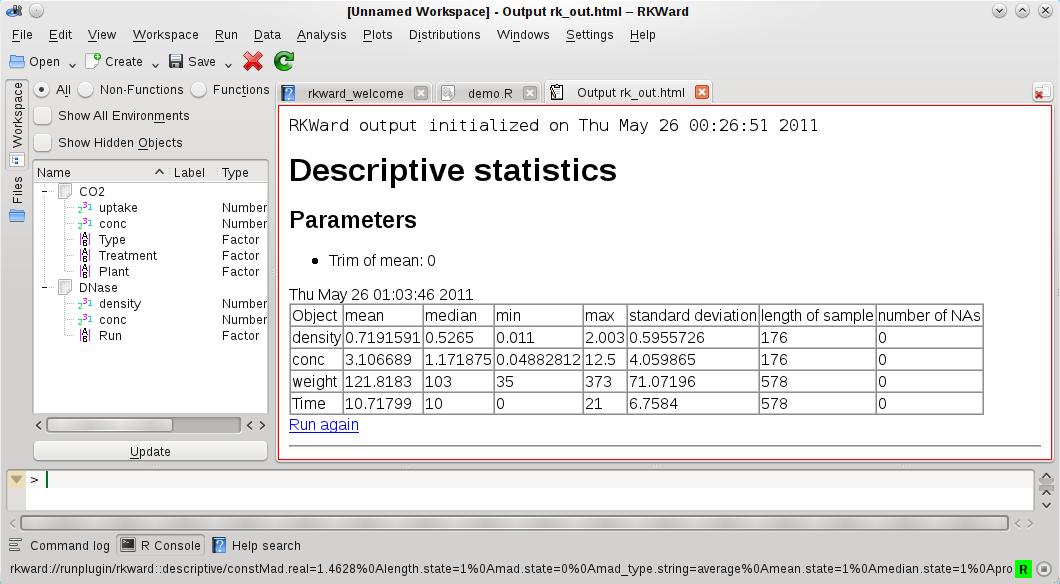
\includegraphics[width=15.5cm]{./figures/results_output_cropped.png}
 \caption{Sample contents of the output window. Upper portion: Result of analyzing sample data (from the
\code{DNase} and \code{ChickWeight}
  datasets of the \pkg{datasets} package) in the ``Descriptive Statistics'' plugin. Standard elements of
  plugin output include a standardized header, and a  ``Run again''-link, which allows to repeat the
  analysis with identical or similar parameters. Lower portion: A custom heading added using the
  \code{rk.header()} function, and a short transcript of R code with corresponding output.}
% TF: Stefan: I've removed the bit below. It was not really designed to allow this, and for the more complex plugins, this is fairly useless,
% since only a fraction of the options will fit in the status bar:
% (Details of the previous analysis are shown in the status bar when the mouse pointer hovers over the ``Run again''-link)
 \label{fig:results_output}
\end{figure}

The formatting of output is kept to a minimum. In particular,
\pkg{RKWard} is very reluctant to round numerical results for the sake of a
pretty output. Rather, the focus is on making the results easily
accessible for further processing, typically in a dedicated word
processor. Output is based on
HTML, and the raw
HTML file and any images therein can be directly
retrieved from a dedicated folder
(by default, this is a folder named ``.rkward'' inside the user's home folder). It is also
possible to select and copy sections of the output directly from the
output window, and to paste them into office applications as
richly formatted text; even images and tables can be easily copied by drag \& drop to many office applications. In future releases, 
it is planned to integrate \pkg{RKWard}
with existing office suites. This
will possibly also mean addition of different file formats such as Open Document Format and technologies such as \pkg{sweave} and \pkg{odfWeave}
\citep{Leisch2002, Kuhn2006}.

Images contained in the output are stored as
portable network graphics (PNG)\footnote{\url{http://www.libpng.org/pub/png/}} by
default, but JPEG\footnote{\url{http://www.jpeg.org/jpeg/index.html}} and
scalable vector graphics (SVG)\footnote{\url{http://www.w3.org/Graphics/SVG/}}
can also be used. Similarly, the size of 
images can be configured by the user. It is expected that SVG will
become the default output format eventually, but currently some SVG
files produced by \proglang{R} are not properly
rendered by older supported versions of the
\pkg{KDE} libraries.

Users can also add custom content to the output window using \code{rk.header()}, \code{rk.print()}, and some
related functions. Further, custom R code as well as the corresponding R output can easily be documented in
the \pkg{RKWard} output window, including syntax highlighting (see the lower portion of
Figure~\ref{fig:results_output}).

\subsection{Package management}
\label{sec:package_management}
The number of \proglang{R} packages available from the comprehensive \proglang{R} archive
network (CRAN), Omegahat\footnote{\url{http://www.omegahat.org/}} and Bioconductor \citep{Gentleman2004} has grown exponentially since \proglang{R}\, 1.3
(2001) to \proglang{R}\, 2.7 (2008) \citep{Fox2008, Ligges2003, Visne2009}. \pkg{RKWard}
utilizes functionality from a growing number of these packages, but avoids
making the installation of all supported packages a pre-requirement to using
\pkg{RKWard} at all. Only once a not yet installed package is required to conduct a certain
action, a package management dialog is invoked automatically, which allows to
download and install the package from a repository such as CRAN. The package
management dialog can also be invoked manually from the menu
(``Settings$\rightarrow$Configure Packages'') for installing new or updating existing \proglang{R}
packages. The underlying package management technology is that of \proglang{R}
\citep{Ligges2003, Ripley2005}.

\pkg{RKWard} supports installing packages to any user writable location. If no current
library location is user writable, \pkg{RKWard} offers to create a new one. 
On UNIX systems, interactively acquiring root privileges for
installation to the system-wide libraries is also supported.
The installation process
itself can be monitored at the interface for error tracking. At the time of this writing, \pkg{RKWard} has no
built-in tools for the interactive exploration of \proglang{R} packages. However, it is
possible to invoke external helpers as reported elsewhere \citep{Zhang2004}.

\subsection{Further tool windows}
\label{sec:further_tool_windows}

The file browser tool window can be
used to open supported file types (e.\,g., \proglang{R}
scripts, HTML files) inside the main \pkg{RKWard}
window. For unsupported file types (such as portable document format; PDF), the
system's default external applications are used.

The command log window contains a log of the commands that have been
evaluated by the \proglang{R} engine, and any output
produced by these commands. By default, the log shows only commands
which have been entered by the user or directly correspond to user
actions, but it can be configured to include commands which are run for
\pkg{RKWard}'s internal purposes such as keeping the workspace browser up
to date.

Commands can be submitted while the \proglang{R} engine
has not yet started, or while another lengthy calculation is still
in progress. In these cases, commands are placed into a queue first, and
executed as soon as the \proglang{R} engine becomes
available. The ``pending jobs'' window (not shown in the tool area by default)
lists current \proglang{R} commands waiting for
evaluation by the \proglang{R} engine. While this
window is mostly of interest to application developers for diagnostic
purposes, it can also be used to interrupt selected commands.

\subsection{Help system}
\label{sec:help_system}

\pkg{RKWard} provides access to both \proglang{R} specific and 
\pkg{RKWard} specific help pages.
\proglang{R} specific documentation includes help pages for functions and packages 
and the various \proglang{R} manuals. \pkg{RKWard} specific documentation consists of
help pages on \pkg{RKWard} in general and on specific GUI dialogs\footnote{For technical 
background of \pkg{RKWard} GUI help pages please refer to the technical supplement to this article.}. 
All these various types of help pages can be browsed in the same document 
window, and can be cross--linked. For example, help pages for
\pkg{RKWard} GUI dialogs will typically link to documentation for both
related \pkg{RKWard} dialogs and the underlying \proglang{R} functions.
An arbitrary number of help windows can be browsed simultaneously, in the
TDI view area (see Figure~\ref{fig:main_window}C) or in detached windows.

A central access point to the help system is the ``Help'' menu. Further, help pages on
\nobreak{\pkg{RKWard}} GUI dialogs can be accessed from the dialog itself using the
``Help'' button. A useful (``reverse'') feature here is that these pages include 
a link near the top of the page to start the corresponding GUI dialog directly.
Help on \proglang{R} specific functions can be invoked from multiple places, 
such as, the context menu of the workspace browser, by pressing F2 (function
reference) while the cursor is on a function name either in the code editor or 
in the \proglang{R} console, and of course, by using the \proglang{R} \code{help()}
command. In addition, a tool view window is provided as an interface to the
\code{help.search()} command in \proglang{R}. This allows to search all installed, 
all loaded, or specific \proglang{R} packages for a specified topic.

The help browser window is based on the \pkg{KDE}
HTML viewer component and supports many standard
features like increasing or decreasing the font size and searching text
within a page. Additionally, \proglang{R} code inside a help
page can be sent to the \proglang{R} engine for
evaluation by selecting it and pressing F8 (or via ``Run$\rightarrow$Run
Selection'').
